\documentclass[aps,prb,reprint,superscriptaddress,longbibliography,floatfix]{revtex4-2}

\usepackage{amsmath,amssymb,bm}
\usepackage{booktabs}
\usepackage{graphicx}
\usepackage{microtype}
\usepackage{xcolor}
\usepackage[colorlinks=true,citecolor=blue!55!black,linkcolor=blue!55!black,urlcolor=blue!55!black]{hyperref}
\hypersetup{pdftitle={Mechanism-Dependent Geometric ETH under Exact Degeneracy},pdfauthor={Thomas J. Wang; OKongOYangO},pdfsubject={Non-Abelian quantum geometry across parent, cohomological, and stabilizer mechanisms}}

% Generated from audited v12 JSON; do not edit numerical values.
\newcommand{\CrossMechanismBranch}{domain\_limited\_geometric\_eth}
\newcommand{\MRParticleSizes}{4,6}
\newcommand{\MRNFourRank}{42}
\newcommand{\MRNSixRank}{120}
\newcommand{\MRNFourBasis}{126}
\newcommand{\MRNSixBasis}{1716}
\newcommand{\MRNFourGap}{1.672850}
\newcommand{\MRNSixGap}{1.535155}
\newcommand{\MRNFourRFour}{0.5016}
\newcommand{\MRNSixRFour}{0.3093}
\newcommand{\MRNFourCumulant}{0.1909}
\newcommand{\MRNFourCumulantSE}{0.0278}
\newcommand{\MRNFourZ}{6.87}
\newcommand{\MRNFourP}{3.13\times 10^{-12}}
\newcommand{\MRNSixCumulant}{0.1936}
\newcommand{\MRNSixCumulantSE}{0.0248}
\newcommand{\MRNSixZ}{7.80}
\newcommand{\MRNSixP}{3.15\times 10^{-15}}
\newcommand{\PanelCount}{24}
\newcommand{\PanelPairCount}{276}
\newcommand{\WickPairingCount}{3}
\newcommand{\LatticeCycleSizes}{1,2,3}
\newcommand{\LatticeRanks}{2,4,8}
\newcommand{\LatticeBasisDims}{9,105,1389}
\newcommand{\LatticeCumulants}{-0.1640,\,-0.1480,\,0.1687}
\newcommand{\LatticePValues}{0.9743,\,0.9994,\,0.0702}
\newcommand{\LatticeCumulantNorms}{0.256,\,0.205,\,0.291}
\newcommand{\XCubeLengths}{2,3,4,5}
\newcommand{\XCubeCurvature}{-0.5}
\newcommand{\XCubeConnectedVariance}{0.0}
\newcommand{\MRNEightBasis}{24,310}
\newcommand{\MRNEightRank}{275}
\newcommand{\MRNEightConstraintNNZ}{44,044,000}
\newcommand{\MRNEightActionProducts}{24,576,552,000}
\newcommand{\MRNTenBasis}{352,716}
\newcommand{\MRNTenRank}{546}
\newcommand{\MRNTenConstraintNNZ}{1,668,086,784}
\newcommand{\MRNTenActionProducts}{1,834,895,462,400}

\newcommand{\Tr}{\operatorname{Tr}}
\newcommand{\cQ}{\mathcal Q}
\newcommand{\cH}{\mathcal H}
\newcommand{\cK}{\mathcal K}

\begin{document}

\title{Mechanism-Dependent Geometric ETH under Exact Degeneracy}

\author{Thomas J. Wang}
\email{WangTheoPhys@outlook.com}
\affiliation{Tsinghua University, Beijing 100084, China}

\author{OKongOYangO}
\affiliation{The Pennsylvania State University, University Park, Pennsylvania 16802, USA}

\date{\today}

\begin{abstract}
Exact degeneracy removes the energy spacings used by conventional quantum-chaos tests but leaves the motion of the degenerate projector over coupling space. We compare this non-Abelian quantum geometry in three many-body mechanisms using one response convention and a covariance-complete fourth cumulant. For the bosonic Moore--Read three-body parent, exact fixed-quasihole zero-mode ranks are \MRNFourRank\ and \MRNSixRank\ at particle numbers \MRParticleSizes. A \PanelCount-panel local-tangent ensemble gives positive normalized directional cumulants \(\MRNFourCumulant\pm\MRNFourCumulantSE\) and \(\MRNSixCumulant\pm\MRNSixCumulantSE\) after all \WickPairingCount\ complex Wick pairings are subtracted. The same registered direction is not positive in a lattice-supersymmetric independence-complex family with ranks \LatticeRanks. In the periodic X-cube code, stabilizer reweighting gives identically zero geometry, whereas local isospectral transport gives scalar curvature \(F=\XCubeCurvature P\) with zero connected variance. These results show that projector motion alone is insufficient for geometric chaos and that the fourth-order response depends on the protection mechanism and perturbation class. We call the resulting finite-size, domain-limited classification Geometric ETH; neither an asymptotic law nor cross-mechanism universality is inferred.
\end{abstract}

\maketitle

\begin{figure*}[t]
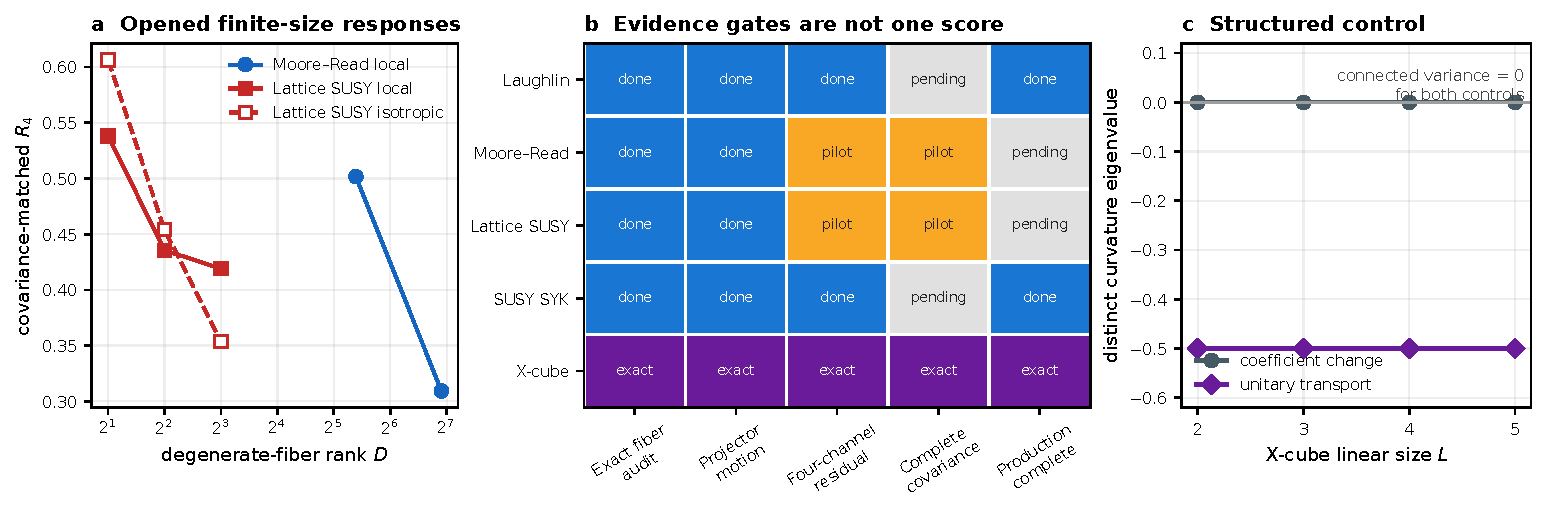
\includegraphics[width=\textwidth]{figures/cross_mechanism_v12.pdf}
\caption{\label{fig:cross}Mechanism-resolved evidence under exact degeneracy. (a) Covariance-matched fourth-order residuals for the opened Moore--Read and lattice-SUSY cases. The lines guide the eye and are not asymptotic fits. (b) Separate exact-fiber, projector-motion, four-channel, complete-covariance, and production gates. The Laughlin and supersymmetric-SYK rows summarize previously opened task artifacts; their different inference protocols are not silently pooled with the present panel U-statistic. Yellow cells are conditional panel results, blue cells are completed calculations, purple cells are exact controls, and gray cells remain pending. (c) X-cube coefficient changes give zero curvature, whereas isospectral transport gives one scalar eigenvalue and zero connected variance.}
\end{figure*}

Energy-level statistics cannot resolve an exactly degenerate eigenspace. This blind spot occurs in supersymmetric sectors, frustration-free parent Hamiltonians, and stabilizer codes for different microscopic reasons. Lifting the degeneracy to recover Wigner--Dyson statistics changes the protected object one intended to study. The alternative is to retain the degeneracy and ask how its projector moves as physical couplings change. Berry and Wilczek--Zee transport make this question gauge covariant \cite{berry1984,wilczekzee1984}; the quantum metric supplies its symmetric counterpart \cite{provostvallee1980,kato1950}.

Chen, Colin-Ellerin, Mamroud, and Papadodimas proposed the non-Abelian Berry curvature of degenerate BPS multiplets as an intrinsic chaos observable and found a contrast between structured smooth microstates and random-matrix-like black-hole sectors \cite{chen2026berry}. This geometric viewpoint does not, by itself, determine which correlation law should hold in condensed-matter zero-mode manifolds. Locality, clustering constraints, cohomology, and stabilizer relations restrict the virtual response channels in different ways. The question here is therefore stronger than whether a curvature spectrum looks random: does a covariance-matched Gaussian law close the fourth moment across independent protection mechanisms?

Let \(P(\bm\lambda)\) project onto a \(D\)-dimensional exactly degenerate eigenspace at energy \(E_0\), and let \(\bar P=1-P\). For a tangent \(\partial_a H\), we use the reduced response
\begin{equation}
X_a=\bar P(H-E_0)^{-1}\bar P(\partial_a H)P.
\label{eq:response}
\end{equation}
Its sign relative to \(\bar P\partial_a P P\) is immaterial below. The matrix-valued quantum geometric tensor and its antisymmetric part are
\begin{equation}
\cQ_{ab}=X_a^\dagger X_b,\qquad F_{ab}=i(\cQ_{ab}-\cQ_{ba}),
\label{eq:qgt}
\end{equation}
while \(g_{ab}=(\cQ_{ab}+\cQ_{ba})/2\). Under a basis rotation within \(P\cH\), these objects transform by conjugation; their spectra and traced contractions are gauge invariant.

For tangent labels \(a,b,c,d\), one response panel gives
\begin{equation}
T_{abcd}=D^{-1}\Tr(X_a^\dagger X_bX_c^\dagger X_d).
\label{eq:fourpoint}
\end{equation}
We whiten the label covariance and compare \(T\) with its covariance-matched Wick tensor. The single-panel ratio \(R_4=\lVert T-T_{\mathrm W}\rVert_F/\lVert T_{\mathrm W}\rVert_F\) measures residual fourth-order structure. For inference across panels, we form a complete U-statistic: the physical tensor is averaged within panels, whereas each of the three complex Wick contractions is estimated from all distinct panel pairs. The registered scalar direction is proportional to \(\delta_{ab}\delta_{cd}+\delta_{ad}\delta_{cb}\); uncertainty comes from delete-one panel pseudovalues. This construction includes the pseudocovariance contraction omitted by a proper-complex two-pairing approximation. It is nevertheless conditional on exchangeability of local tangent panels at a fixed Hamiltonian, not an independent Hamiltonian or disorder ensemble.

We implement three exact-degeneracy mechanisms. The continuum lowest-Landau-level Moore--Read parent \cite{mooreread1991,zhang2023parent} is factorized as
\begin{equation}
H_{\mathrm{MR}}=\sum_x C_x^\dagger C_x,\qquad C_x=\frac{1}{\sqrt{3!}}\left(\sum_j\phi_{xj}b_j\right)^3,
\label{eq:mrparent}
\end{equation}
where \(x\) runs over a complete magnetic-translation orbit of coherent states. We use the fixed-four-quasihole sequence \(N_\phi=N+2\) and guiding-center-density tangents. The lattice-supersymmetric family uses constrained fermion creation on a disjoint union of \(m\) six-site cycles \cite{fendley2003lattice,huijse2010cohomology},
\begin{equation}
Q(\bm z)=\sum_i z_i c_i^\dagger\prod_{j\sim i}(1-n_j),\qquad H_{\mathrm{SUSY}}=\{Q,Q^\dagger\},
\label{eq:susyparent}
\end{equation}
in charge sector \(2m\). Nilpotency identifies the zero modes with independence-complex cohomology and gives rank \(2^m\). The X-cube Hamiltonian is a commuting stabilizer sum on the three-torus \cite{vijay2016xcube}; its ground-space dimension is \(2^{6L-3}\). Positive coefficient changes keep its projector fixed. A separate two-parameter unitary conjugation moves the projector isospectrally and supplies an analytic structured control.

Figure~\ref{fig:cross} separates the evidence gates. For Moore--Read, every exact-kernel, internal-bandwidth, external-gap, residual, and response check passes. The fiber ranks are \(D=\MRNFourRank,\MRNSixRank\), with external gaps \(\MRNFourGap,\MRNSixGap\). The median local residual decreases from \(R_4=\MRNFourRFour\) to \(\MRNSixRFour\), but two sizes do not define a scaling law. More importantly, the covariance-complete fixed-direction estimates are \(\MRNFourCumulant\pm\MRNFourCumulantSE\) and \(\MRNSixCumulant\pm\MRNSixCumulantSE\), with one-sided \(p=\MRNFourP\) and \(p=\MRNSixP\), respectively. Each estimate uses all \PanelPairCount\ unordered pairs of \PanelCount\ panels.

The lattice-SUSY calculation passes nilpotency, exact/coexact branch reconstruction, response, gap, and kernel checks at \(m=\LatticeCycleSizes\), with ranks \(D=\LatticeRanks\). Its normalized fixed-direction estimates are \(\LatticeCumulants\), with one-sided \(p\)-values \(\LatticePValues\). None passes the registered positive-direction gate. The full normalized cumulant norms, \(\LatticeCumulantNorms\), remain nonzero; thus the result is a failure of transfer of one direction, not a proof of Gaussianity.

The X-cube controls resolve a logical ambiguity. Reweighting fixed commuting stabilizers changes energies but not \(P\), so \(g=F=0\) exactly. For local generators \(G=X_e/2\) and \(K=iX_eS/2\), where \(S\) is a vertex-plane stabilizer containing edge \(e\), unitary transport preserves the full spectrum and gap but gives
\begin{equation}
iP[\partial_G P,\partial_K P]P=-\frac{1}{2}P.
\label{eq:xcubecurvature}
\end{equation}
The projector moves and the Berry curvature is nonzero, yet the connected curvature variance vanishes. Nontrivial geometry is therefore not sufficient for random geometric mixing.

These three mechanisms rule out two overly broad statements. Exact degeneracy does not make quantum geometry trivial, because the Moore--Read and lattice-SUSY projectors have resolved response and the X-cube transport has nonzero curvature. Conversely, projector motion does not imply geometric chaos, because Eq.~\eqref{eq:xcubecurvature} is completely scalar. The fourth moment further distinguishes the positive Moore--Read direction from the lattice-cohomology family. The natural classification is therefore relative to both the protection mechanism and the chosen perturbation algebra.

We use the term \emph{Geometric ETH} for the program of replacing energy-resolved chaoticity by statistical closure of gauge-covariant response tensors on an exactly degenerate fiber. The present branch, \texttt{\CrossMechanismBranch}, is deliberately domain limited. It establishes finite-size mechanism dependence and a necessary counterexample to ``moving projector implies chaos.'' It does not establish conventional ETH \cite{srednicki1994}, thermalization, a Lyapunov exponent, a thermodynamic limit, a universal scaling function, or inference from independent Moore--Read Hamiltonians. The disjoint-cycle SUSY graph is an exactly controlled cohomological family rather than a generic connected material, and the X-cube paths are analytic interventions rather than stochastic ensembles.

The next decisive calculation is not a larger collection of unrelated models. It is a controlled thermodynamic test inside at least two mechanisms with matched ensemble units. The staged Moore--Read \(N=8\) case and a connected lattice-SUSY family can determine whether the positive cumulant persists, changes direction, or closes toward a mechanism-specific Gaussian law. Until those tests are complete, the scientific conclusion is mechanism-dependent quantum geometry under exact degeneracy, not a universal Geometric ETH theorem.

\begin{acknowledgments}
The numerical artifacts, exact-rank audits, panel-pair tensors, and source hashes are retained with the reproducibility package. We thank the Quantum Harness community for discussions about fail-closed numerical claims.
\end{acknowledgments}

\bibliography{references}

\end{document}
